\documentclass[a4paper,12pt]{article} % тип документа

%  Русский язык
\usepackage[T2A]{fontenc}			% кодировка
\usepackage[utf8]{inputenc}			% кодировка исходного текста
\usepackage[english,russian]{babel}	% локализация и переносы

\usepackage{graphicx, scalerel}               % импорт изображений
\usepackage{wrapfig}                % обтекаемые изображения
\graphicspath{{pictures/}}          % обращение к подкаталогу с изображениями
\usepackage[14pt]{extsizes}         % для того чтобы задать нестандартный 14-ый размер шрифта
\usepackage[warn]{mathtext}         % русский язык в формулах
\usepackage{indentfirst}            % indent first
\usepackage[margin = 25mm]{geometry}% отступы полей
\usepackage[table,xcdraw]{xcolor}   % таблицы
\usepackage{amsmath,amsfonts,amssymb,amsthm,mathtools} % Математика
\usepackage{wasysym}                % ???
\usepackage{upgreek}                % ???  
\usepackage{caption}
\usepackage{multirow}
\captionsetup{labelsep=period}
\usepackage[font=small,labelfont=bf]{caption}
\usepackage{gensymb} % degree symbol
\usepackage{tikz}
\usetikzlibrary{positioning}


\begin{document}
	
	
	\begin{center}
		
		\textbf{НАЦИОНАЛЬНЫЙ ИССЛЕДОВАТЕЛЬСКИЙ УНИВЕРСИТЕТ \\ <<МОСКОВСКИЙ ФИЗИКО-ТЕХНИЧЕСКИЙ ИНСТИТУТ>>}
		\vspace{13ex}
		
		\textbf{Лабораторная работа 4.7.3\\ <<Изучение поляризованного света>>}
		\vspace{40ex}
		
		\normalsize{Шумаков Иван Игоревич \\ студент группы Б01-009\\ 3 курс ФРКТ\\}
	\end{center}
	
	\vfill 
	
	\begin{center}
		г. Долгопрудный\\ 
		2022 г.
	\end{center}
	
	
	\thispagestyle{empty} % выключаем отображение номера для этой страницы
	\newpage
	
	
	\textbf{Цель работы:} исследовать модель АЧТ; измерить постоянные Стефана-Больцама и Планка по излучению накаленных тел.
	\textbf{В работе используются:} оптический пирометр, модель АЧТ, исследуемые тела, вольтметры.


	\section{Теоретические сведения}

		Для измерения температуры разогретых тел, удалённых от наблюдателя, применяют методы оптической пирометрии, основанные на использовании зависимости испускательной способности исследуемого тела от температуры. Различают три температуры, функционально связанные с истинной термодинамической температурой и излучательной способностью тела: радиационную $T_{rad}$, цветовую $T_{col}$ и яркостную $T_{br}$. \par
		В работе измеряется яркостная температура. \textbf{Яркостная температура} - это температура абсолютно чёрного тела, при которой его спектральная испускательная способность равна спектральной испускательной способности исследуемого тела при той же длине волны.
		Измерение яркостной температуры раскалённого тела производится при помощи оптического пирометра с исчезающей нитью, основанного на визуальном сравнении яркости раскалённой нити с яркостью изображения исследуемого тела. \par
		Яркостная температура тела всегда ниже его термодинамической температуры. Это связано с тем, что любое нечёрное тело излучает меньше, чем АЧТ при той же температуре. Зависимость между яркостной и термодинамической температурами вольфрама приведена на рис. 1
		\begin{figure}[h]
			\centering
			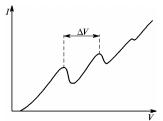
\includegraphics[width=10cm]{img/fig2.PNG}
			\caption{График зависимости $T = f(T_{br})$ для вольфрам}
			\label{ris:fig1}
		\end{figure}
		По результатам измерений мощности излучения вольфрамовой нити можно судить о справедливости закона Стефана-Больцмана. Если бы нить излучала как АЧТ, то баланс потребляемой и излучаемой энергии определялся бы соотношением 
		\begin{equation}
			W = \sigma S (T^4 - T_0^4),
		\end{equation}
		где $W$ - потребляемая нитью электрическая мощность, $S$ - площадь излучающей поверхности нити, $T$ - температура нити, $T_0$ - температура окружающей среды. Однако вольфрамовая нить излучает как серое тел, и излучение её ослаблено по сравнению с АЧТ в $\varepsilon_T$ раз для любой волны при данной температуре тела Т. Тогда предположив, что нить излучает как серое тело и с учётом того, что $T_0 \ll T$, выражение (1) можно переписать в виде
		\begin{equation}
			W = \varepsilon_T S \sigma T^4
		\end{equation}
		В справедливости закона Стефана-Больцмана можно убедиться, построив график зависимости $W(T)$ в логарифмическом масштабе и по углу наклона определить показатель степени $n$ исследуемой температурной зависимости. В пределах погрешности показатель степени должен быть близок к четырём. \par
		Также из формулы (2) можно определить постоянную Стефана-Больцмана.


	\section{Экспериментальная установка}

		\begin{figure}[h]
			\centering
			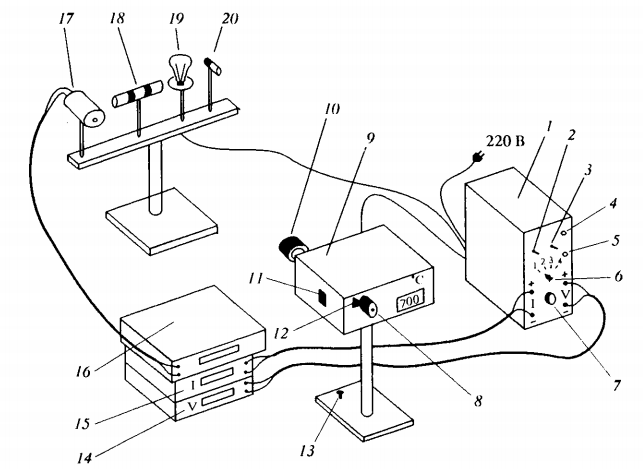
\includegraphics[width=11cm]{img/fig1.PNG}
			\caption{Схема экспериментальной установки: 1 - блок питания; 2 - тумблер включения питания образцов; 3 - тумблер нагрева нити пирометра; 4 - кнопка "Нагрев нити"; 5 - кнопка "охлаждение нити"; 6 - тумблер переключения образцов; 7 - регулятор мощности нагрева образцов; 8 - окуляр пирометра; 9 - корпус пирометра; 10 - объектив пирометра; 11 - переключение диапазонов; 12 - ручка смещения красного светофильтра; 13 - регулировочный винт; 14 - вольтметр (напряжение на лампе накаливания); 15 - амперметр (ток через образцы); 16 - вольтметр в цепи термопары; 17 - модель АЧТ; 18 трубка с кольцами из материалов с различной излучательной способностью; 19 - лампа накаливания; 20 - неоновая лампочка}
			\label{fig2}
		\end{figure}
		Исследуемые в работе образцы:
		\begin{itemize}
			\item \textbf{модель абсолютно чёрного тела} - керамическая трубка, закрытая с одного конца и окружённая для теплоизоляции внешним кожухом. Температура в трубке измеряется с помощью термопары хромель-алюмель
			\item \textbf{керамическая трубка с набором колец из различных материалов}, нагреваемая изнутри нихромовой спиралью. Материалы колец имеют различную излучательную способность
			\item \textbf{вольфрамовая нить электрической лампочки}
		\end{itemize}
	\newpage


	\section{Ход работы}

		\subsection{Изучение работы оптического пирометра}
		
			В данном пункте была проверена калибровка пирометра. 
			Для этого была измерена яркостная температура модели АЧТ с помощью термопары и с помощью пирометра.
			Измеренные данные:
			\begin{equation}
				T_{real} = 1012 [^oC] \hspace{10mm}
				T_{exper} = 978 [^oC] 
			\end{equation}
			Относительная погрешность пирометра равна:
			\begin{equation}
				\delta_{\text{пир}} = \frac{34}{978} = 0.03
			\end{equation}
			
		\subsection{Измерение яркостной температуры накаленных тел}

			При измерении яркостной температуры накаленных тел их свечение было недостаточно сильным, поэтому различная светимость была определена невооруженным глазом.\par
			Таким образом было подтверждено, что различные тела, нагретые до одинаковых температур, имеют различные яркостные тмпературы.
		
		\subsection{Проверка закона Стефана-Больцама}

			Для проверки закона Стефана-Больцмана были измерены мощность, потребляемая лампой, и её температуры. 
			Для этого были получены значения тока через нить, напряжение на ней и её яркостная температура.\par		
			\begin{table}[h!]
				\centering
				\begin{tabular}{|l|l|l|}
				\hline
				$T_{bright} [C^{0}]$				  & U [мВ] & I [A]     \\ \hline
				900                                   & 19.3       & 0.65  \\ \hline
				100                                   & 21.9       & 0.68  \\ \hline
				1100                                  & 29.5       & 0.774 \\ \hline
				1200                                  & 34.04      & 0.83  \\ \hline
				1300                                  & 41.7       & 0.91  \\ \hline
				1400                                  & 50.8       & 1.008 \\ \hline
				1500                                  & 63.76      & 1.132 \\ \hline
				1600                                  & 72.39      & 1.21  \\ \hline
				1700                                  & 83.7       & 1.31  \\ \hline
				1800                                  & 94.9       & 1.4   \\ \hline
				1700                                  & 83.8       & 1.35  \\ \hline
				1600                                  & 73.9       & 1.22  \\ \hline
				1500                                  & 63.9       & 1.134 \\ \hline
				1400                                  & 53.3       & 1.03  \\ \hline
				1300                                  & 54.5       & 0.94  \\ \hline
				1200                                  & 38.3       & 0.87  \\ \hline
				1100                                  & 30.8       & 0.78  \\ \hline
				1000                                  & 23.9       & 0.64  \\ \hline
				900                                   & 18.7       & 0.63  \\ \hline
				\end{tabular}
			\end{table}
			Вычисление показателя степени температуры:
			\begin{equation}
				W = \epsilon_TBT^n
			\end{equation}
			\begin{equation}
				ln{W} = ln(\epsilon_TB) + n ln{T}
			\end{equation}
			При построении графика яркостная температура сначала была переведа в Кельвины и затем в температуру нити в соответствии с рисунком \ref{ris:fig1}.
	\newpage

			\begin{figure}[h]
				\centering
				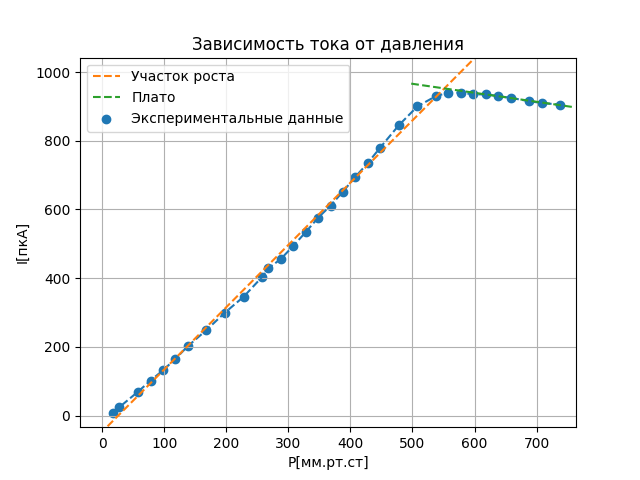
\includegraphics[width=15cm]{img/Graph1.PNG}
				\caption{Зависимость мощности от температуры в логарифмическом масштабе}
				\label{graph1}
			\end{figure}
			При анализе всех полученных данных коэффициент $k = 4.25$ и случайная погрешность $\delta_k \approx 0.01$.\par
			При анализе температур свыше $1300 [^oC]$ коэффициент $k = 4.02$, но из-за малого количества данных случайная погрешность возрастает до $\delta_k \approx 0.04$.\par
			Второе значение ближе к теоретическому, поскольку при более высоких температурах накаленная нить ближе к модели серого тела.\par
			Таким образом с учетом погрешности пирометра показатель степени Т равен:
			\begin{equation}
				\delta_n = \delta_k + 4 * \delta_T = 0.01 + 4 * 0.03 \approx 0.1
			\end{equation}
			\begin{equation}
				n = 4.0 \pm 0.4				
			\end{equation}
			Полученные данные подтверждают закон Стефана-Больцмана.\par
	\newpage
			В форрмулах выше коэффициент $B$ выражается как:
			\begin{equation}
				B = S * \sigma
			\end{equation} 
			\begin{equation}
				S = 0.36 [\text{см}^2] - \text{площадь излучающей поверхности нити}
			\end{equation}
			\begin{equation}
				\sigma - \text{постоянная Стефана-Больцмана}
			\end{equation}
			Таким образом:
			\begin{equation}
				\sigma = \frac{W}{\epsilon_T ST^4}
			\end{equation}
			С помощью этой постояной можно найти постоянную Планка:
			\begin{equation}
				h =\sqrt[3]{\frac{2 \pi^5 k_\text{Б}}{15 c^2 \sigma}}
			\end{equation}
			График зависимости постоянной Планка от температуры нити:
			\begin{figure}[h]
				\centering
				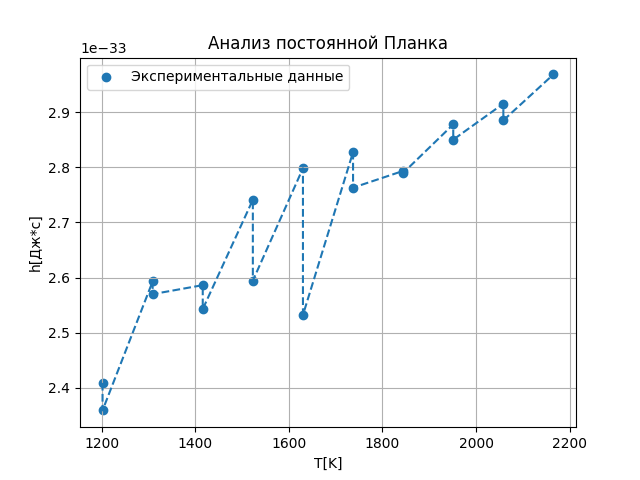
\includegraphics[width=15cm]{img/Graph2.PNG}
				\caption{Зависимость постоянной Планка от температуры}
				\label{graph2}
			\end{figure}
			Значения постоянной Планка сильно отличаются друг от друга в зависимости от температуры.
			Из этого можно сделать вывод, что модель серого тела применима к вольфрамовой нити только в узком диапазоне температур.
			Оценим постоянную Планка как 
			\begin{equation}
				h \approx 28 * 10^{-34} [\text{Дж  с}]
			\end{equation}
			С учетом разброса значений и погрешности $\sigma$ ($\delta_\sigma = 4 * \delta_T \approx 0.1$) оценим погрешность $h$ как:
			\begin{equation}
				\delta_h \approx 0.2
			\end{equation}
			Таким образом постоянная Планка равна:
			\begin{equation}
				h = (28 \pm 5.6) * 10^{-34} [\text{Дж с}]
			\end{equation}
			Расхождение с табличным значением $h = 6.62 * 10{-34} [\text{Дж с}]$ менее одного порядка.

		\subsection{Измерение яркостной температуры неоновой лампочки}

			С помощью пирометра была измерена яркостная температура неоновой лампочки:
			\begin{equation}
				T = 847 [^oC]
			\end{equation}
			Ее реальная температура примерно равна комнатной.
			Такое различие реальной и яркостной температуря обусловлено тем, что в спектр неоновой лампы обусловлен спектром излучения неона за счет перехода атомов на другие энергетические уровни,
			а не тепловым излучением.
		
	\section{Выводы}
			
		В данной работе было исследовано тепловое излучение различных тел. 
		На основе полученных данных, был проверен закон Стефана-Больцама и вычислена постоянная Планка.\par
		Закон Стефана-Больцмана был подтвержден с высокой точностью. 
		Теоретическое значение лежит в пределах погрешности.\par
		Постоянная Планка получилась в 4 раза болше теоретической. 
		Это может быть связано с тем, что нить не до конца соответствует модели серого тела. 
		Также возможно ошибка связана с неправильным значением константы $S$.  
	
\end{document}